%-*- coding: UTF-8 -*-
\documentclass[hpyerref,UTF8,a4paper,titlepage,12pt,oneside]{ctexbook}
\usepackage{hyperref}
\usepackage{geometry}
\usepackage{xeCJK, fontspec, xunicode, xltxtra,ulem}
\usepackage{amsthm}
\usepackage{amsmath}
\usepackage{amssymb}
\usepackage{mathrsfs}
\usepackage{mathtools}
\usepackage{commath}
\usepackage{listings}
\usepackage{float}
\usepackage{xcolor}
\usepackage{mdframed}

% \graphicspath{{../images/}}
\geometry{a4paper,bottom=2cm}

\title{Qiaternions and Rotation}
\author{陈国庆}
\date{\today}

\bibliography{plain}

% 定理结构
\theoremstyle{definition}
\newtheorem{definition}{定义}[section]
\newtheorem{theorem}{定理}[section]
\newtheorem{corollary}{推论}[theorem]
\newtheorem{lemma}[theorem]{Lemma}
\renewcommand\qedsymbol{$\blacksquare$}

\begin{document}

\maketitle
\tableofcontents

\section{三维空间旋转}

平面上向量绕原点旋转一个角度,可通过向量与单位复数的乘积来表示,比如向量$v= [x,y]$,逆时针旋转$\theta$后的向量可表示为,
$$
	v^\prime = (x + iy)\cdot (\cos \theta + i\sin\theta)
$$

展开结果又可以表示为$2\times 2$矩阵,
$$
	v^\prime = \begin{bmatrix}
		\cos\theta,& -\sin\theta\\
		\sin\theta,& \cos\theta
	\end{bmatrix}
	\begin{bmatrix}
		x\\
		y
	\end{bmatrix}
$$

这也是线性代数里的结果,上述矩阵称为\textit{旋转矩阵}。\\

三维空间中,绕$z$轴旋转,相当于只改变$xy$而$z$值不变,对应的矩阵为,
$$
	R_z(\theta) = \begin{bmatrix}
			&\cos\theta,&-\sin\theta, & 0\\
			&\sin\theta,&\cos\theta, &0\\
			&0,&0,&1
		\end{bmatrix}
$$

对应的,在$zx$平面绕$y$轴旋转,
$$
	R_y(\theta) = \begin{bmatrix}
			&\cos\theta,&0, &\sin\theta\\
			&0, &1,&0\\
			&-\sin\theta,&0,&\cos\theta\\
		\end{bmatrix}
$$
以及,在$yz$平面绕$x$轴旋转,
$$
	R_x(\theta) = \begin{bmatrix}
			&1,	&0,			&0\\
			&0, &\cos\theta,&-\sin\theta\\
			&0,	&\sin\theta,&\cos\theta\\
		\end{bmatrix}
$$
 
很快发现,$R_y$与$R_x,R_z$对称性并不相同,这并非错误,是因为我们默认用了\textit{右手坐标系},假定逆时针是沿着$x-y-z-x$的顺序,所以$zx$平面相对$z$轴旋转$\theta$,相当于$xz$平面相对$x$轴旋转$-\theta$。

\begin{figure}[H]
	\begin{center}
		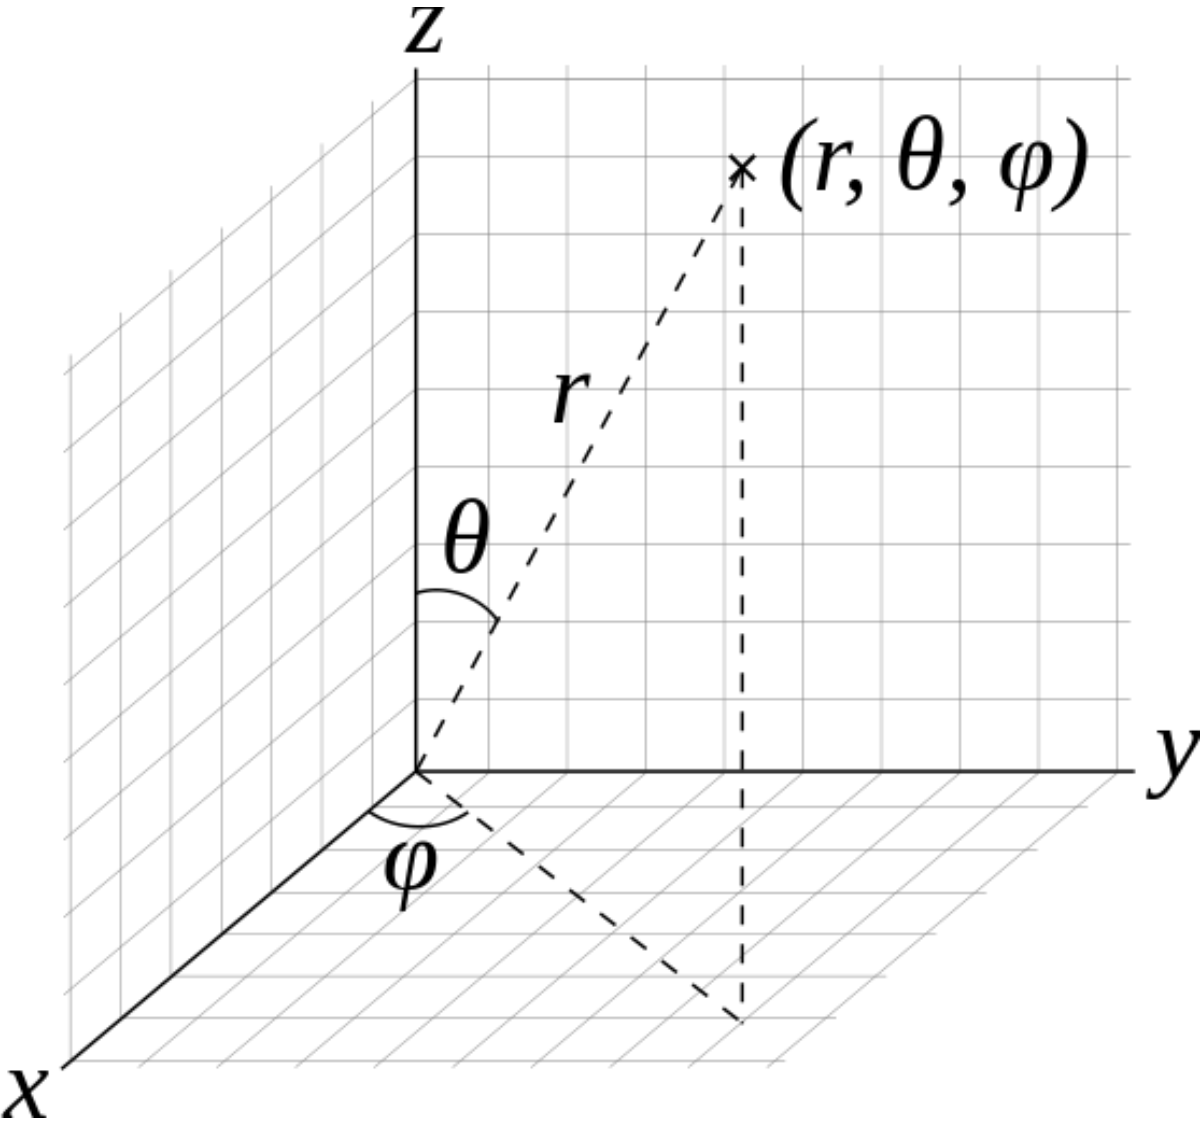
\includegraphics[width=0.8\textwidth]{./images/righthandless.png}
		\caption{右手坐标系}
	\end{center}
\end{figure}


旋转矩阵是单位正交矩阵,存在一些很好的性质,
$$
	R^{-1} = R^T, \quad R(\theta)R(-\theta) = I,\quad R(-\theta)=R^{-1}(\theta)
$$

那向量$\mathbf{v}$绕单位向量$\mathbf{n}$的旋转该如何表示?\\

\begin{figure}[H]
	\begin{center}
		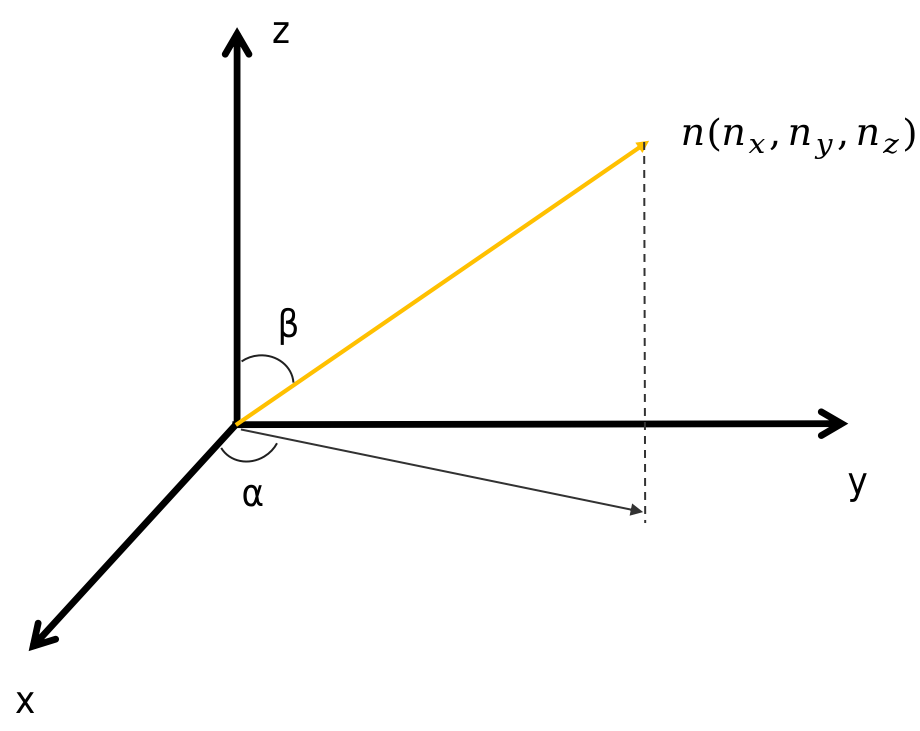
\includegraphics[width=0.8\textwidth]{./images/axis_rotation.png}
	\end{center}
\end{figure}

如上图,分三步操作:
\begin{itemize}
	\item 将$xy$平面绕z轴\textit{逆时针}旋转$\alpha$,再将$zx$平面绕y轴\textit{逆时针}旋转$\beta$,使得$\mathbf{n}$与z轴重合
	\item $\mathbf{v}$绕z轴\textit{逆时针}旋转$\theta$
	\item 将坐标系旋转回原位置
\end{itemize}

如此可直接写出旋转矩阵,
$$
	R_{\mathbf{u}}(\theta) = R_z(\alpha)R_y(\beta)R_z(\theta)R_y(-\beta)R_z(-\alpha)
$$

$\alpha,\beta$可用$\mathbf{n}$的坐标表示,得到最终展开形式,
$$
	R_{\mathbf{u}}(\theta) = \begin{bmatrix}
	&\cos \theta +n_x^2(1-\cos\theta), &n_xn_y(1-\cos\theta)-n_z\sin\theta,&n_xn_z(1-\cos\theta) +n_y\sin\theta\\
	&n_yn_x(1-\cos\theta) + n_x\sin\theta, &\cos\theta + n_y^2(1-\cos\theta),&n_yn_z(1-\cos\theta) - n_x\sin\theta\\
	&n_zn_x(1-\cos\theta) -n_y\sin\theta, &n_xn_y(1-\cos\theta) +n_x\sin\theta,&\cos\theta+n_z^2(1-\cos\theta)
	\end{bmatrix}
$$

将矩阵拆开重新组合可得\textit{罗德里格斯}公式,
\begin{equation}\label{rodrigues}
	\mathbf{v}^\prime = (1-\cos\theta)(\mathbf{v}\cdot\mathbf{n})\mathbf{n} + \cos\theta\cdot\mathbf{v} + \sin\theta\cdot(\mathbf{n}\times \mathbf{v})
\end{equation}

\section{四元数}
用矩阵表示旋转,二维空间的$2\times 2$矩阵,对应到三维空间是$3\times 3$矩阵,是一个很自然的扩展过程;\\

复数也对应着旋转,是否存在三元复数代表三维空间的旋转?\\

对此,哈密尔顿马上就进行了尝试,引入两个虚数单位$\mathbf{i}^2 = -1,\mathbf{j}^2 = -1$,定义了一个三元数
$$
	\mathbf{v} = v_0 + v_1 \mathbf{i} +v_2 \mathbf{j}
$$

计算一下两个三元数$\mathbf{v},\mathbf{u}$的乘积,
\begin{align*}
	\mathbf{v}\cdot\mathbf{u} 
		&= (v_0 + v_1 \mathbf{i} +v_2 \mathbf{j})(u_0 + u_1 \mathbf{i} +u_2 \mathbf{j}) \\
		&= v_0u_0 + (v_0u_1 + v_1u_0)\mathbf{i} +(v_0u_2 +v_2u_0)\mathbf{j} -v_1u_1 -v_2u_2 + (v_1u_2)\mathbf{i}\mathbf{j} + (v_2u_1)\mathbf{j}\mathbf{i}
\end{align*}

此时出现$\mathbf{i}\mathbf{j},\mathbf{j}\mathbf{i}$,这两个值应该如何定义?

\begin{itemize}
	\item 若$\mathbf{i}\mathbf{j}=0 \Rightarrow \mathbf{i}^2 = 0$,与定义矛盾
	\item 若$\mathbf{i}\mathbf{j}=r(r\ne 0)\Rightarrow \mathbf{i}=-r\mathbf{j}$,两个虚数相互表示,构不成三元数
	\item 若$\mathbf{i}\mathbf{j}=\mathbf{i}\Rightarrow \mathbf{j} = 1$,与定义矛盾
\end{itemize}

也就是在现有数系下,$\mathbf{i}\mathbf{j}$无法定义。汉密尔顿扩展数域,又引入了第三个虚数$\mathbf{k}$,可定义如下,
\begin{align*}
	&i^2 = j^2 = k^2 = ijk= -1\\
	&ij=k,jk=i,ki =j\\
	&ij=-ji,jk=-kj,ki=-ik
\end{align*}

这就是就是\textit{四元数}。很明显,四元数放弃了交换律。\\

对四元数
$$
	p = p_0 +p_1 \mathbf{i} +p_2 \mathbf{j} +p_3 \mathbf{k}, \quad q = q_0 +q_1 \mathbf{i} +q_2 \mathbf{j} +q_3 \mathbf{k}
$$

对应的积,
\begin{align*}
	pq = p_0q_0 &- (p_1q_1 + p_2q_2 +p_3q_3) +p_0(q_1\mathbf{i} +q_2\mathbf{j} + q_3 \mathbf{k}) +q_0(p_1 \mathbf{i} + p_2 \mathbf{j} + p_3 \mathbf{k})\\
		& +(p_2q_3 -p_3q_2)\mathbf{i} +(p_3q_1 -p_1q_3)\mathbf{j} + (p_1q_2 - p_2q_1)\mathbf{k}
\end{align*}

用内积叉积表示为,
\begin{align}\label{quatern_multiple}
	pq &= p_0q_0 - \mathbf{p}\cdot \mathbf{q} +p_0 \mathbf{q} +q_0 \mathbf{p} + \mathbf{p} \times \mathbf{q}\\
	qp &= p_0q_0 - \mathbf{p}\cdot \mathbf{q} +p_0 \mathbf{q} +q_0 \mathbf{p}  - \mathbf{p} \times \mathbf{q}
\end{align}

$pq$与$qp$确不对称,差异在最后一项叉积方向不同。\\

定义复共轭,
$$
	q^* = q_0 -( q_1 \mathbf{i} +q_2 \mathbf{j} +q_3 \mathbf{k})
$$

常把后三项合一起,
$$
	q = q_0 + \mathbf{q}, \quad q^* = q_0 - \mathbf{q}
$$

如此$\mathbf{q}$代表三维空间,$q_0$代表第四个维度;当$q_0=0$时,$q$是一个三维向量,称为\textit{纯四元数}。\\

以此类推,也可定义逆元、模等,相比二元复数除了乘法不满足交换律,其他性质也都具备。\\

单位四元数是模为1的四元数,满足
$$
	q_0^2 +\Vert \mathbf{q}\Vert = 1
$$

存在$\theta \in[0,\pi]$,
$$
	\cos^2\theta = q_0^2, \quad \sin^2\theta = \Vert q\Vert
$$

令$\mathbf{u} = \mathbf{q}/\Vert q\Vert$,对$\mathbf{q}$归一化,则单位四元数可记为,
$$
	q = \cos\theta +  \mathbf{u}\sin\theta
$$

\subsubsection*{四元数旋转变换}

重点来了,单位四元数
$$
	q = \cos\frac{\theta}{2} + \mathbf{u}\sin\frac{\theta}{2}
$$

以及任意的三维向量$\mathbf{v}$,定义变换$L_q$

\begin{equation}
	L_q(\mathbf{v}) = q\mathbf{v}q^*\label{quaternion_rotation}
\end{equation}

变换结果为$\mathbf{v}$绕$\mathbf{u}$逆时针旋转$\theta$。\\

证明一下这个结论\footnote{\url{https://graphics.stanford.edu/courses/cs348a-17-winter/Papers/quaternion.pdf}},根据(\ref{quatern_multiple})展开(注意$\mathbf{v}$是纯四元数),
	\begin{align*}
		L_q(\mathbf{v}) 
			&= q \mathbf{v}q^*\\
			& = (-\mathbf{q} \cdot \mathbf{v} + q_0 \mathbf{v} + \mathbf{q}\times \mathbf{v})(q_0 - \mathbf{q})\\
			&= -q_0(\mathbf{q}\cdot \mathbf{v}) 
				+ (q_0 \mathbf{v} + \mathbf{q}\times \mathbf{v})\cdot\mathbf{q} 
				+ (\mathbf{q}\cdot \mathbf{v})\mathbf{q}
				+ q_0(q_0 \mathbf{v} + \mathbf{q}\times \mathbf{v})
				- (q_0 \mathbf{v} + \mathbf{q}\times \mathbf{v}) \times \mathbf{q}\\
			&= (q^2_0 - \Vert \mathbf{q}\Vert^2)\mathbf{v} + 2(\mathbf{q}\cdot \mathbf{v})\mathbf{q} +2q_0(\mathbf{q}\times \mathbf{v})\\
			&= \left( \cos^2\frac{\theta}{2} - \sin^2\frac{\theta}{2}\right)\mathbf{v}
				+ 2\left(\mathbf{u} \sin\frac{\theta}{2}\cdot \mathbf{v}\right) \mathbf{u} \sin\frac{\theta}{2}
				+ 2\cos\frac{\theta}{2}\left( \mathbf{u} \sin\frac{\theta}{2} \times \mathbf{v}\right)\\
			&= \cos\theta\cdot \mathbf{v} + (1 -\cos\theta)(\mathbf{u}\cdot \mathbf{v})\mathbf{u} +\sin\theta\cdot(\mathbf{u}\times \mathbf{v})
	\end{align*}

	这是(\ref{rodrigues})描述的\textit{罗德里格斯公式},旋转矩阵和四元数是\textit{罗德里格斯公式}的两种展开形式,二者是等价的。\\

	相比四元数,矩阵的表示旋转更为直观,工程中用的也较多,但四元数的发现过程,启发了\textit{非交换代数}的研究。\\

	仅对\textbf{纯四元数},$L_q$可解释为三维空间的旋转;对一般的四元数,还不能这么说,因为四维空间中还未定义“旋转”。\\

	所以,任何对四元数旋转的直观解读都是徒劳,比如把四维空间拆分成两个二维空间进行讨论,我们无法直观理解四维空间,无论是拆分还是合并,更何况四维空间还没有旋转这个概念。\\

	对比非交换矩阵空间,$PAP^{-1}$是$A$的相似矩阵,虽没有几何直观,但知道一些性质,比如特征值、迹,不变;若$P$是正交矩阵,模不变。\\

	有这些空间性质就足以刻画相似变换,对$L_q$的理解也应如此。

\section{可除代数及其同构}
	为什么无法定义三元数?这是一个很有意思的问题,我们先说结论\footnote{\url{https://badger.math.uconn.edu/divalg3.pdf}}:\\

		\textit{对\textbf{可除代数},只有$\mathbb{R},\mathbb{C},\mathbb{H},\mathbb{O}$四种,分别为实数、复数、四元数、八元数,并且四元数满足结合律但不满足交换律,八元数满足交换律不满足结合律。}\\

	所以,不存在奇数元数及八元以上的数,当然这是在\textbf{可除代数}的约束下。

	\subsubsection*{代数}
		对一个\textit{有限维}向量空间$A$,以及一个数域$\mathbf{F}$,在$A$上定义一个双线性映射$m: A \times A \rightarrow A$,满足
		\begin{align*}
			m(x,\lambda y+ z) &= \lambda m(x,y) + m(x,z)\\
			m(\lambda x +y, z) &= \lambda m(x,z) + m(y,z)
		\end{align*}

		则向量空间A及映射m一起称为“代数”,记为$(A,m)$

	\subsubsection*{可除代数}
		如果$xy = 0_A \Rightarrow x=0 \text{ or } y=0, \forall x,y \in A$,则$(A,m)$称为\textit{可除代数}\\

		很明显,\textit{可除代数}才支持两边约分。

	\subsubsection*{代数性质}
 		\begin{itemize}
	 		\item \textit{交错(alternative)},$x(xy) = (xx)y, x(yy) = (xy)y, \forall x,y \in A$
	 		\item \textit{结合(associative)},$x(yz) = (xy)z$
	 		\item \textit{交换(commutative)},$xy = yx$
	 		\item \textit{单位元(unital)},存在单位元$1$,满足$x1 = x = 1x$
 		\end{itemize}

 		$\mathbb{R},\mathbb{C}$满足上面所有性质,所以也称为\textit{交换代数},满足交换一定满足交错,反之不然,四元数、八元数都称为\textit{交错代数}。

 	\subsubsection*{同构}
 		两个代数$(A,m),(B,n)$之间建立一个映射$\phi$,如果满足,
 		$$
 			\phi(m(x,y))  = n(\phi(x),\phi(y))
 		$$

 		也就是两个代数运算是一一对应的,比如实数域上定义加法和乘法两种运算,定义指数映射$f(x) = e^x$,则
 		$$
 			e^{x+y} = e^x \cdot e^y
 		$$

 		则$(\mathbb{R},+)$与$(\mathbb{R},\cdot)$在指数映射下同构。同构代数具有完全相同的结构,会认为是“完全一样”。\\


 	我们修正下结论:\textit{在同构意义下,可除代数只有$\mathbb{R},\mathbb{C},\mathbb{H},\mathbb{O}$}\\

 	结论证明繁琐但不困难,请大家直接阅读参考材料即可;文中给出八元数的定义规则,通过图完成,非常有意思,

	\begin{figure}[H]
		\begin{center}
			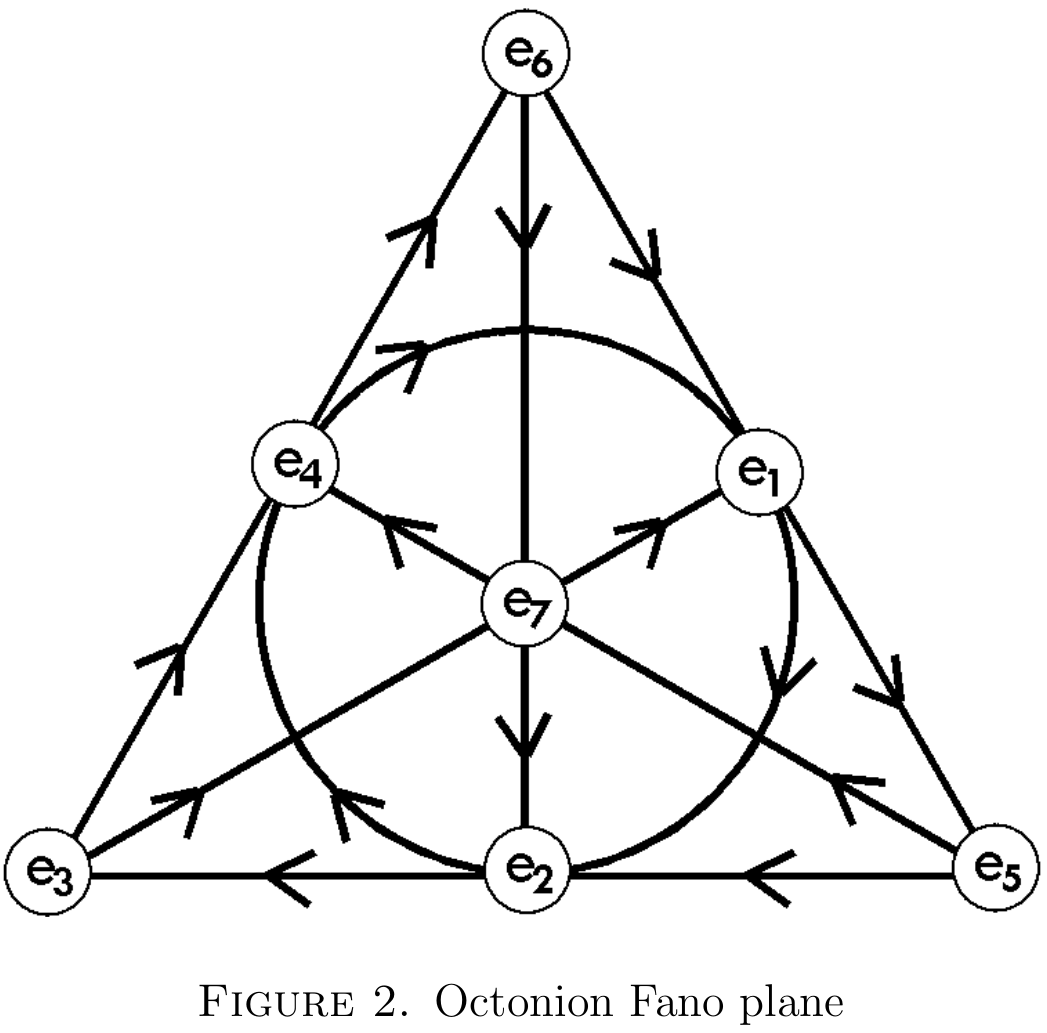
\includegraphics[width=0.8\textwidth]{./images/octnions.png}
		\end{center}
	\end{figure}

	计算法则为,两个数如果按箭头顺序相乘,第三个数在同一直线或同一圆上,结果为正;否则结果为负,比如
	$$
		e_2e_5 = e_3,e_4e_3 = -e_6
	$$
\bibliography{math}
\end{document}